\documentclass[a4paper,12pt]{article}

\usepackage{../usfdvl}


\title{Worksheet 9}
\SetDocumentFooter{}{}


\begin{document}

\maketitle

\worksheetGroundRules


\vspace{5pt}
\section{Assignment}

\begin{itemize}



\item For the following point set, perform:
\begin{enumerate}
\item k-means clustering ($k=3$, you pick initial centers randomly; iterate until convergence)
\item hierarchical clustering (including the resulting tree)
\end{enumerate}
Show the algorithms using as many copies of the following page as needed. Be sure to show all of the steps and the order of steps for the algorithm. Your answer doesn't need to be exactly correct, but be as precise as reasonably possible.

\begin{center}
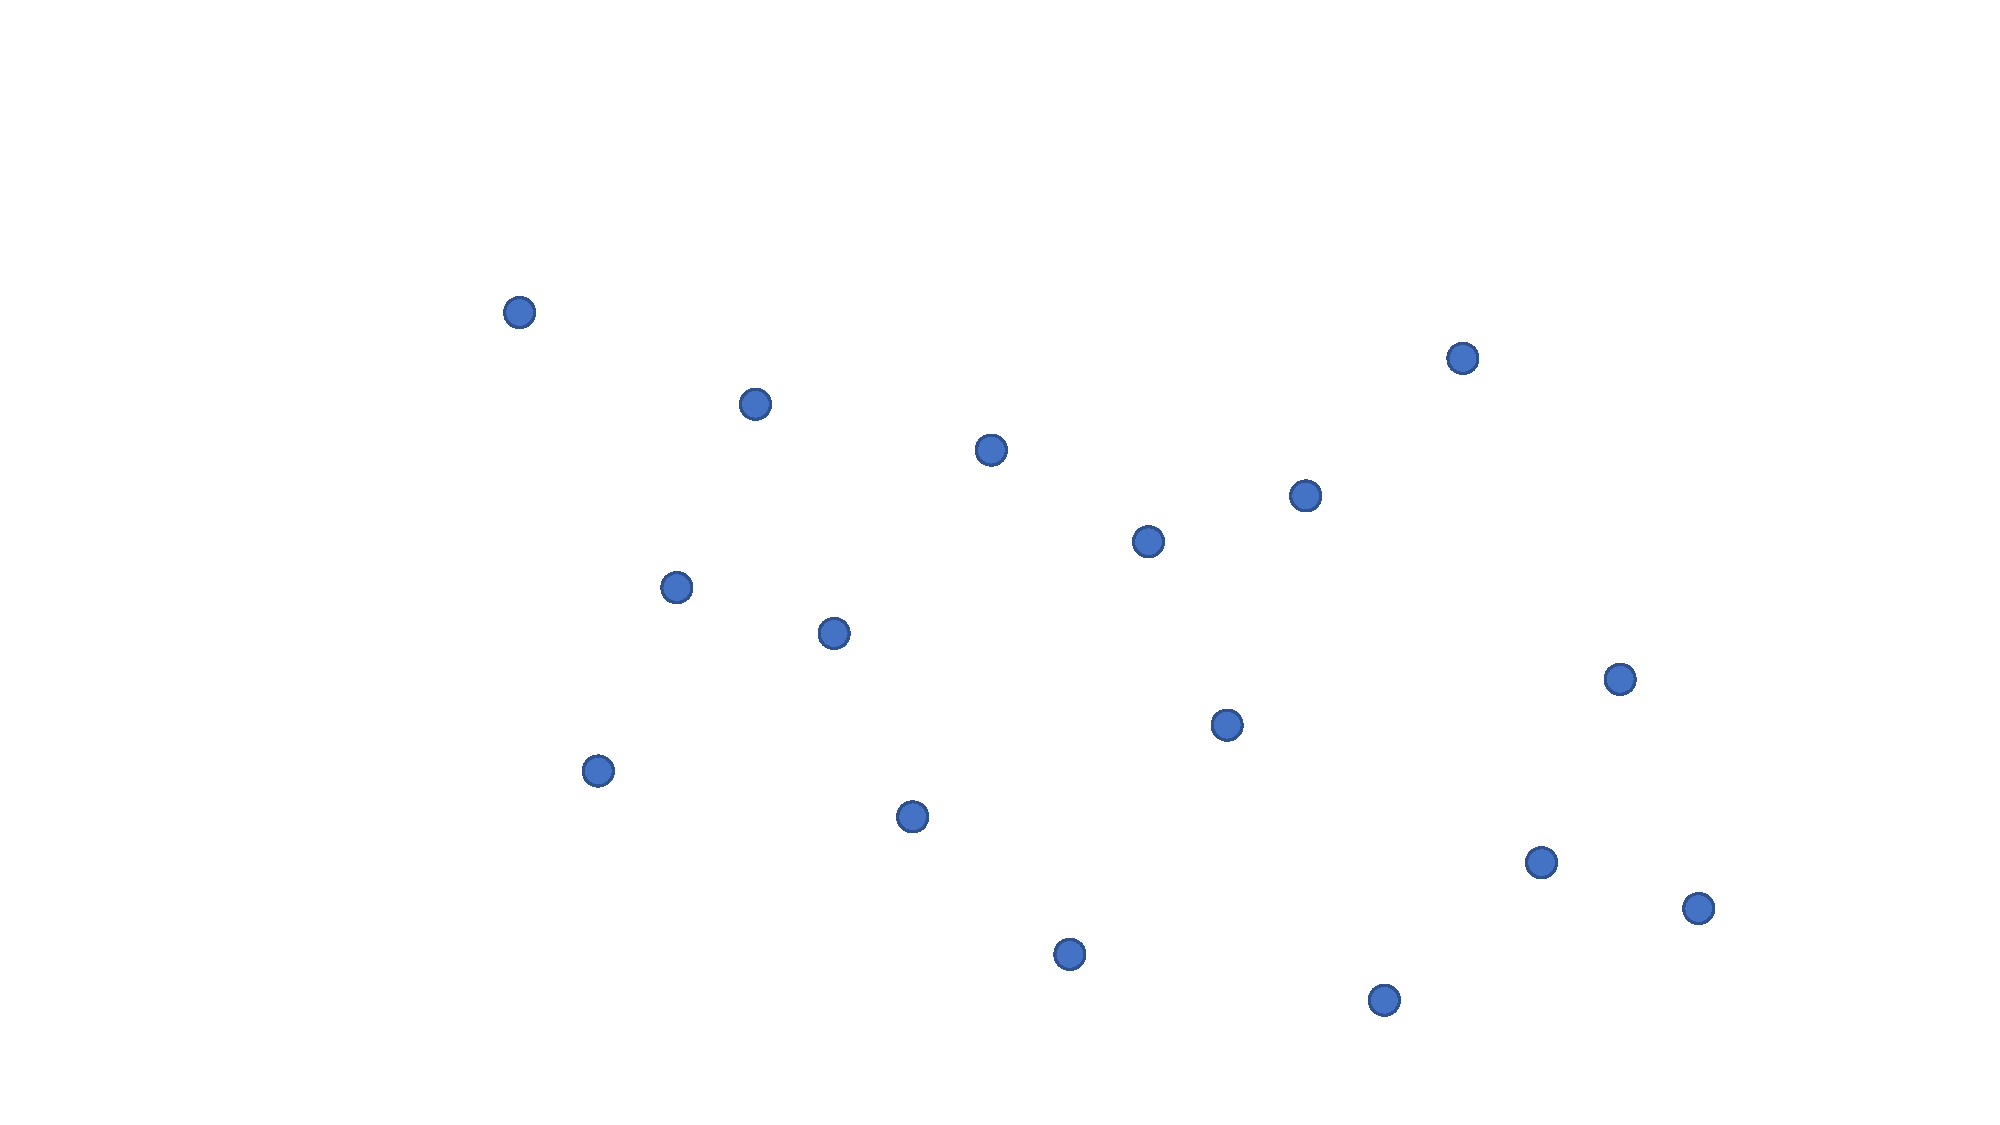
\includegraphics[width=9.5cm]{../images/spatial_subd.pdf}
\end{center}



\end{itemize}


\worksheetSubmission




\newpage

\begin{center}
\begin{tabular}{|c|c|}
\hline
 & \\
\hspace{10pt}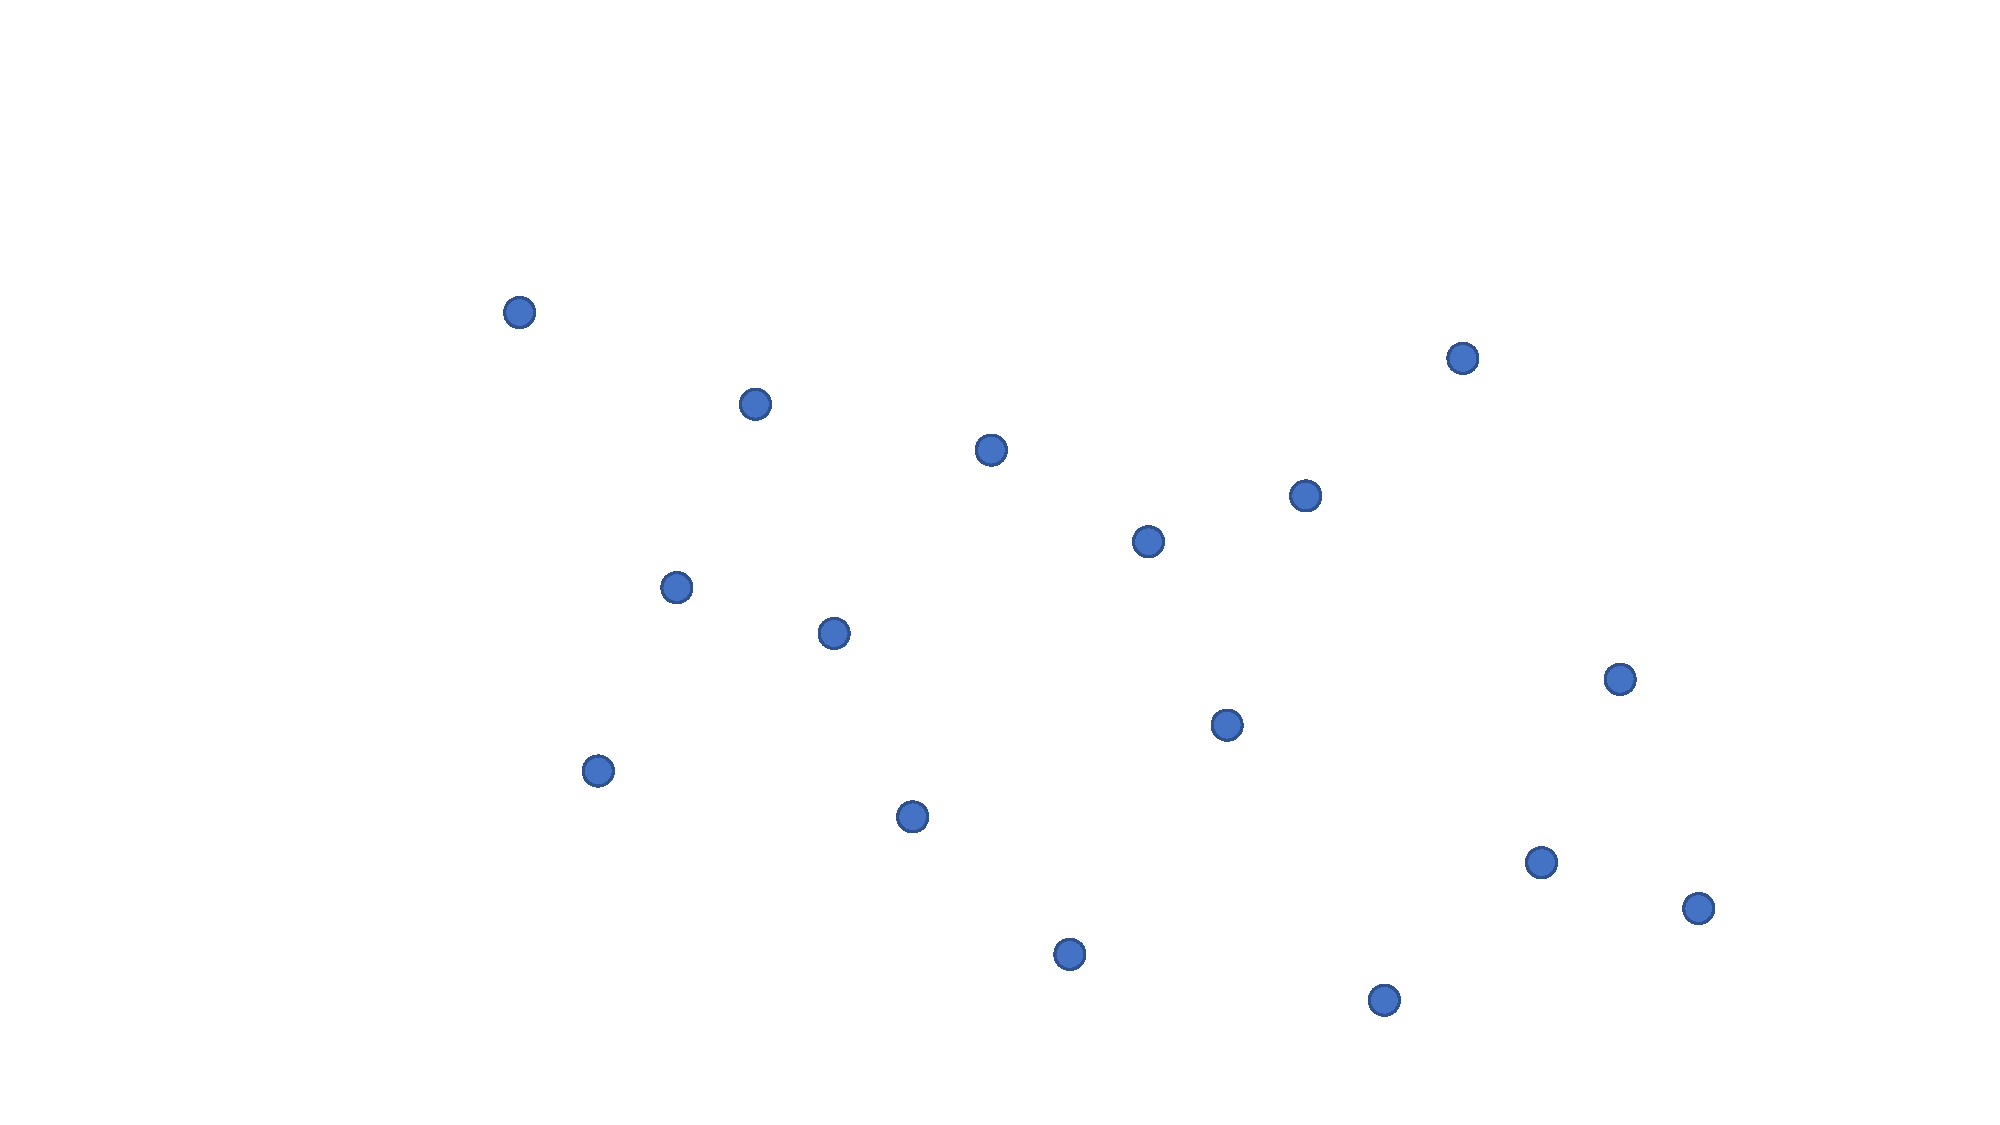
\includegraphics[width=7.5cm]{../images/spatial_subd.pdf}
\hspace{10pt} & \hspace{175pt} \\
 & \\
\hline
 & \\
\hspace{10pt}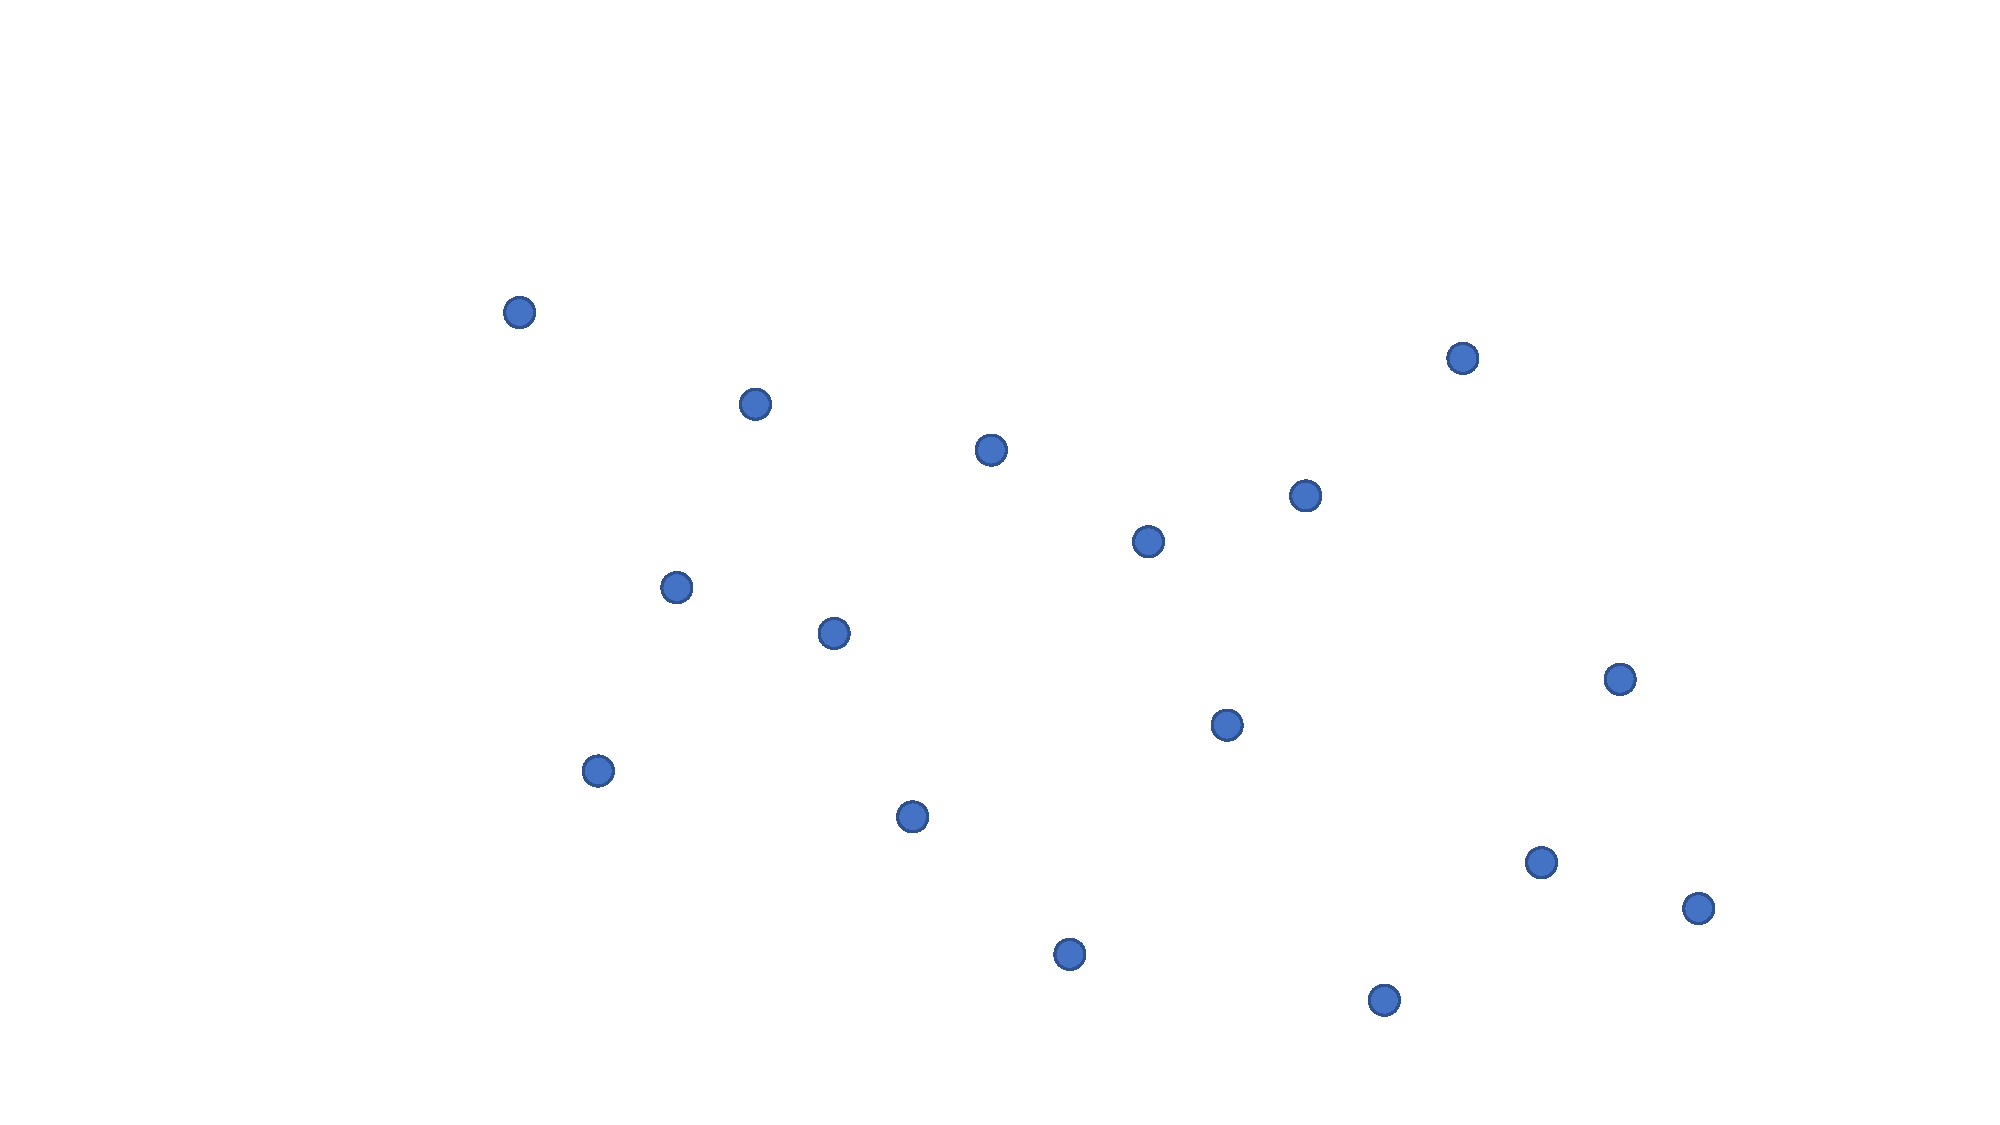
\includegraphics[width=7.5cm]{../images/spatial_subd.pdf}
\hspace{10pt} & \hspace{10pt} \\
 & \\
\hline
 & \\
\hspace{10pt}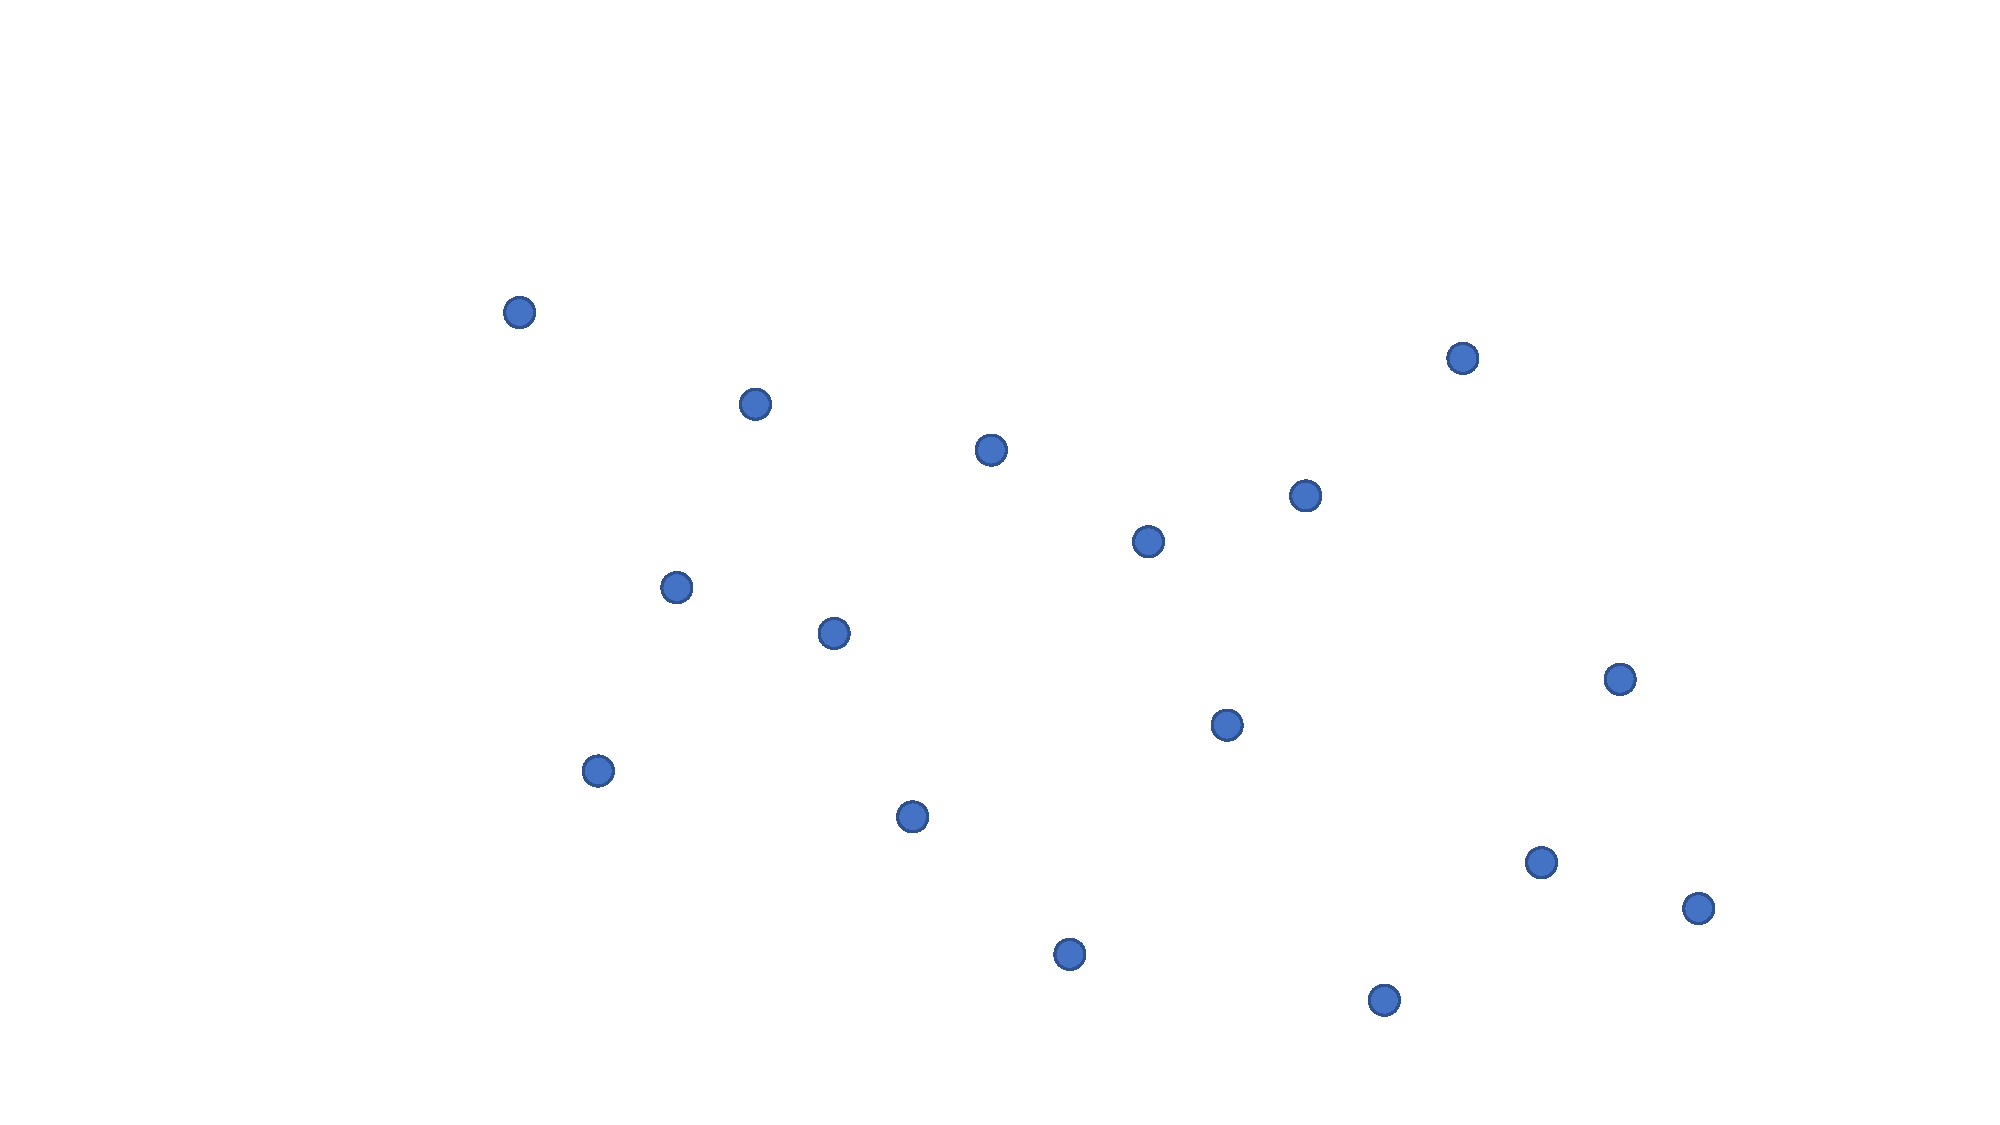
\includegraphics[width=7.5cm]{../images/spatial_subd.pdf}
\hspace{10pt} & \hspace{10pt} \\
 & \\
\hline
 & \\
\hspace{10pt}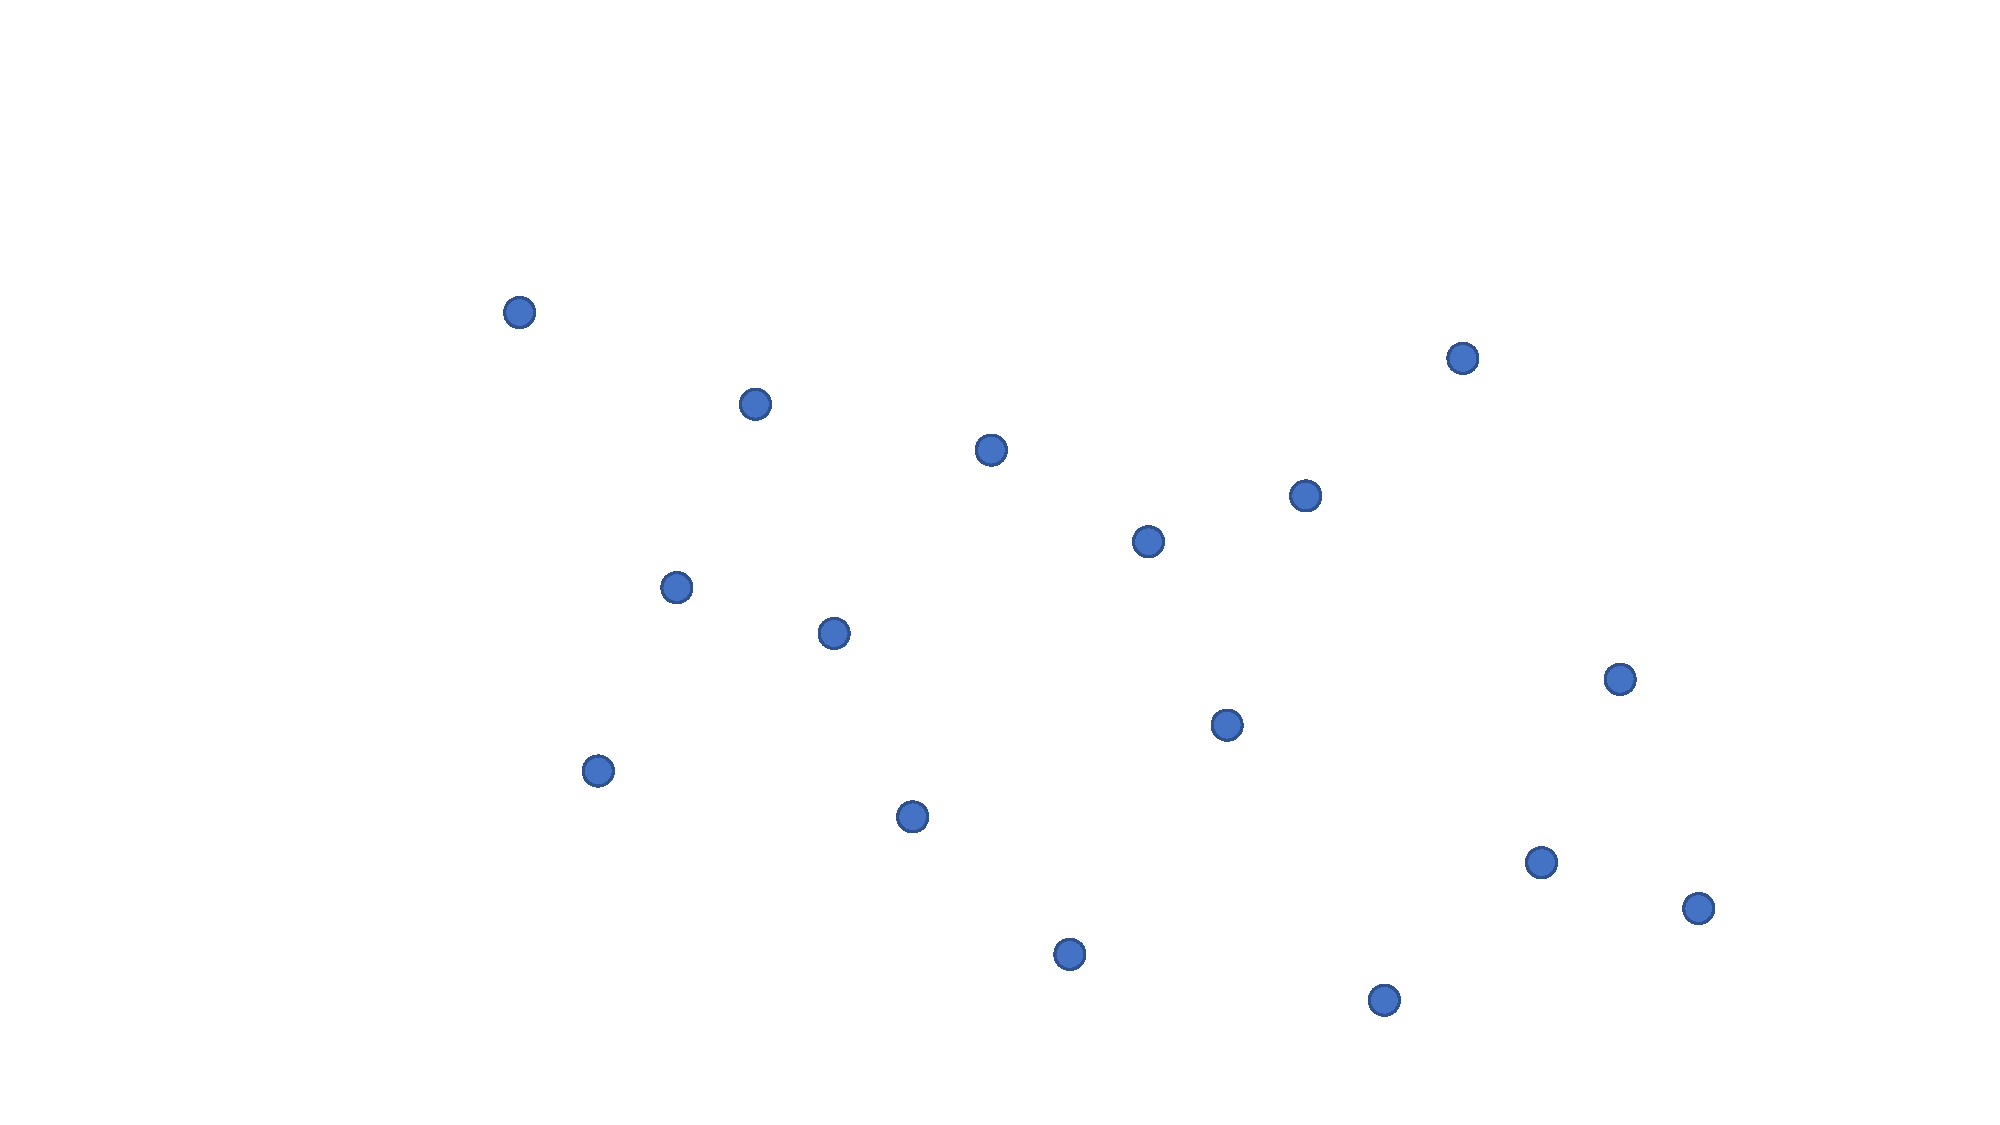
\includegraphics[width=7.5cm]{../images/spatial_subd.pdf}
\hspace{10pt} & \hspace{10pt} \\
 & \\
\hline
\end{tabular}
\end{center}


\end{document}



